%
% section 1.2.2
%
\setcounter{section}{2}
\setcounter{subsection}{1}
\subsection{Το Μοντέλο Δικτύωσης TCP/IP}
Το ARPANET είναι ο πρόγονος του σημερινού Internet.

\begin{inthebox}
\emph{Τι σημαίνει ARPANET;} Είναι τα αρχικά των λέξεων Advanced Research Projects Agency Network.
Το ARPA είναι μια υπηρεσία του υπουργείου Άμυνας των ΗΠΑ που ασχολείται -- όπως λέει και το όνομα του --
με προχωρημένα ερευνητικά προγράμματα. Ένα από αυτά ήταν και η δημιουργία ενός δικτύου με πολλά από τα χαρακτηριστικά του σημερινού Internet, το οποίο ονομάστηκε ARPANET.\\
\end{inthebox}

Το δίκτυο αυτό χρηματοδοτήθηκε κατά κύριο λόγο από το υπουργείο Άμυνας των ΗΠΑ
στα τέλη της δεκαετίας του 60. Κύριος στόχος του ήταν η διασύνδεση μεταξύ τους
πολλών διαφορετικών συστημάτων και δικτύων με διαφανή τρόπο και δυνατότητα να παραμένει
σε λειτουργία ακόμα και αν μεγάλα τμήματα του έβγαιναν εκτός λειτουργίας. Το ARPANET είναι
από τα πρώτα δίκτυα που χρησιμοποίησε μεταγωγή πακέτων.

\begin{figure}[!ht]
  \centering
  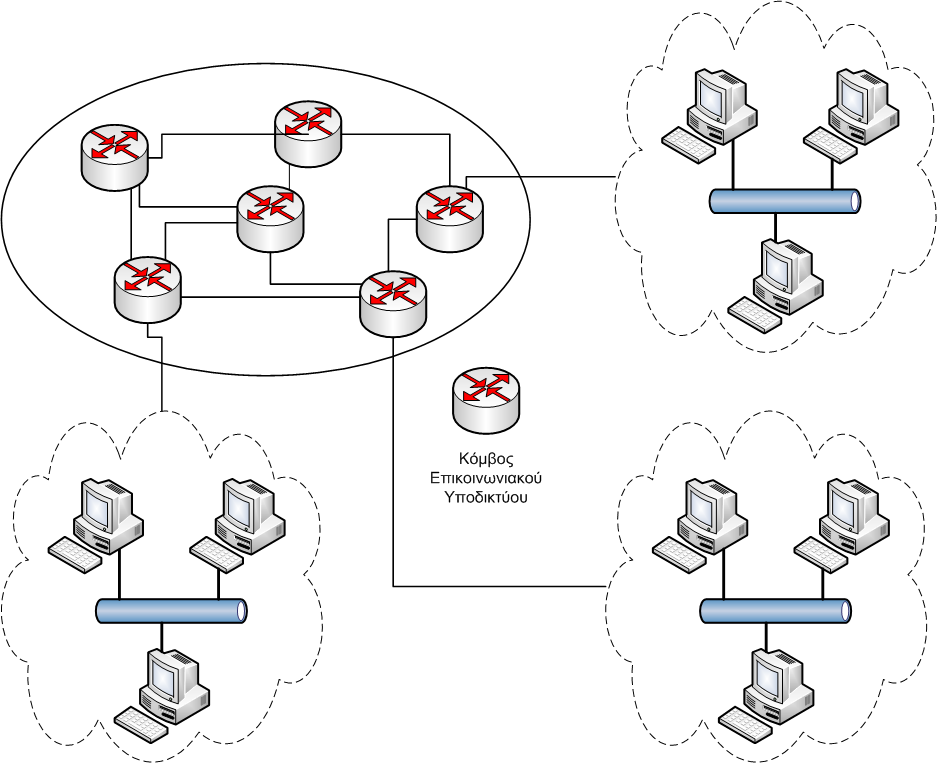
\includegraphics[width=0.95\textwidth]{images/chapter1/1-2}
  \caption {\textsl{Δίκτυο Μεταγωγής Πακέτων}}
  \label{1-2}
\end{figure}

\begin{inthebox}
\emph{Τι είναι η μεταγωγή πακέτων; Τι είναι μεταγωγή γενικά;}
Η λέξη μεταγωγή προέρχεται από το ρήμα ``μετάγω'' που σημαίνει μεταφέρω ή μετακινώ.
Ένα δίκτυο που περιγράφεται ως μεταγωγής πακέτων μεταδίδει την χρήσιμη πληροφορία αφού πρώτα
την κόψει σε μικρότερα κομμάτια (πακέτα) καθένα από τα οποία περνάει από μια σειρά ενδιάμεσων σταθμών
(κόμβων) μέχρι να φτάσει στον προορισμό του, όπως φαίνεται στο σχήμα \ref{1-2}

Το ενδιαφέρον εδώ είναι ότι οι ενδιάμεσοι σταθμοί είναι συνδεδεμένοι μεταξύ τους
με πολλούς τρόπους (υπάρχουν περισσότερες από μία διαδρομές για να πάμε από
ένα σημείο Α σε ένα Β). Εκτός από την μεταγωγή πακέτων, υπάρχει και η μεταγωγή
κυκλώματος η οποία χρησιμοποιείται για τις τηλεφωνικές συνομιλίες στο κλασικό
τηλεφωνικό δίκτυο.

Στη μεταγωγή κυκλώματος ο αποστολέας και ο παραλήπτης συνδέονται απευθείας με
μια γραμμή (αγωγό), τυπικά μόνο για όση διάρκεια κρατάει η επικοινωνία. Για
παράδειγμα, όταν παίρνουμε ένα τηλέφωνο το τηλεφωνικό κέντρο συνδέει απευθείας
(με φυσικό κύκλωμα) την τηλεφωνική μας συσκευή με αυτή που καλούμε. Δεν
υπάρχουν ενδιάμεσοι σταθμοί και η επικοινωνία ξεκινά με την εγκαθίδρυση της
σύνδεσης (όταν ο συνομιλητής μας σηκώσει το ακουστικό!) Στο τέλος της
συνομιλίας μας το τηλεφωνικό κέντρο αποσυνδέει το κύκλωμα το οποίο μπορεί να
χρησιμοποιηθεί για άλλη σύνδεση.

Προφανώς στη μεταγωγή κυκλώματος κάθε σύνδεση μπορεί να χρησιμοποιηθεί μόνο
για μια συνομιλία, ενώ στη μεταγωγή πακέτων οι ενδιάμεσοι κόμβοι μπορούν να
δρομολογούν πακέτα που προέρχονται από διαφορετικούς αποστολείς και
κατευθύνονται σε διαφορετικούς παραλήπτες. Όπως θα δούμε παρακάτω, το πακέτο
περιέχει τις πληροφορίες που χρειάζεται ο κόμβος για να το στείλει στον
προορισμό του.
\end{inthebox}

Για την λειτουργία του ARPANET επιλέχθηκε το 1983 η οικογένεια πρωτοκόλλων
TCP/IP και το δίκτυο σταδιακά εξελίχθηκε στο Internet που γνωρίζουμε σήμερα.

Το TCP/IP είναι μια οικογένεια πρωτοκόλλων με τα δύο βασικότερα, το TCP και το
IP να δίνουν και το κύριο όνομα του. Το TCP/IP χρησιμοποιεί \emph{διαστρωματωμένη
αρχιτεκτονική}, χωρίζεται δηλ. σε επίπεδα (στρώματα) με τρόπο αντίστοιχο με
αυτόν που προτείνεται από το πρότυπο OSI, αλλά χρησιμοποιεί μόνο τέσσερα (4)
επίπεδα αντί για επτά (7). Υπάρχει σε γενικές γραμμές μια (όχι απόλυτη) αντιστοιχία
των επιπέδων του TCP/IP με αυτά του OSI, που φαίνεται στο σχήμα \ref{1-1}.

\begin{figure}[!ht]
  \centering
  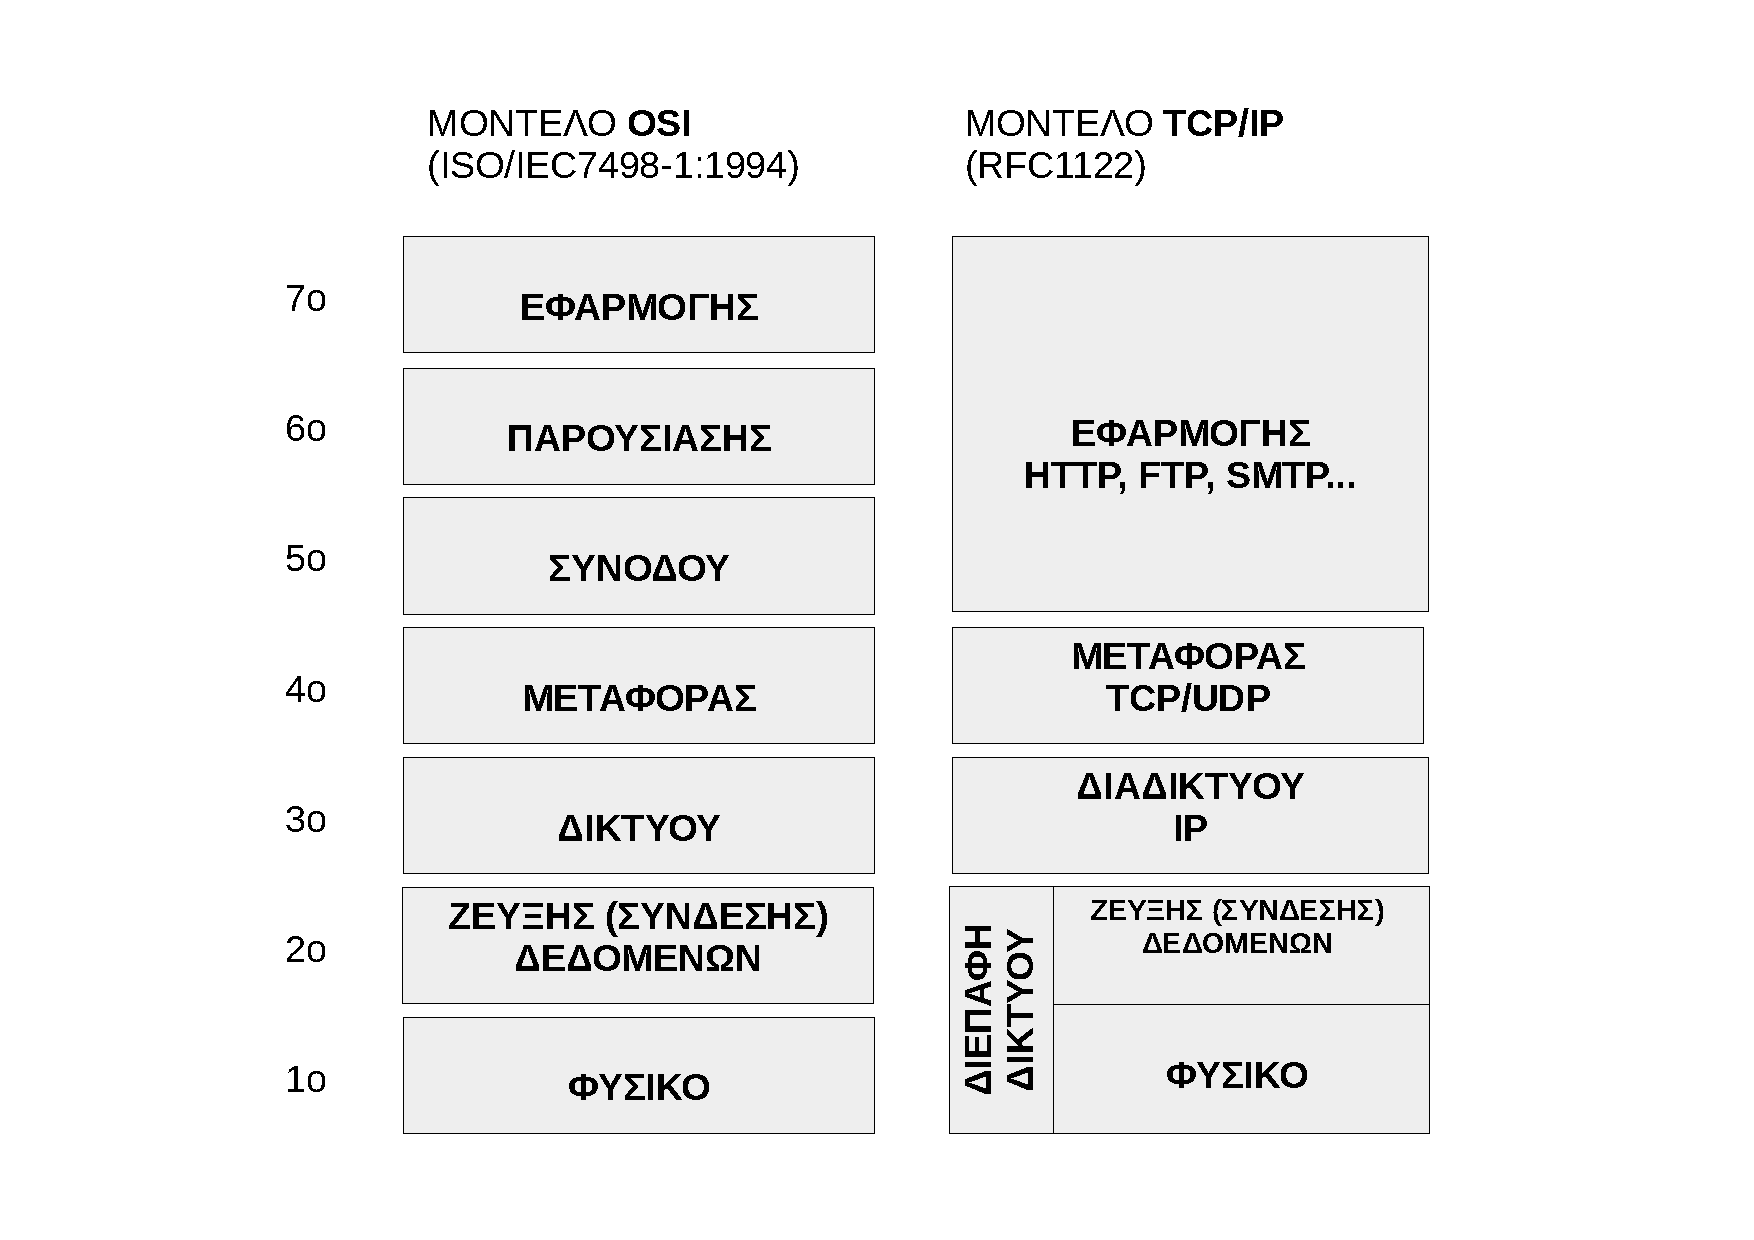
\includegraphics[width=0.95\textwidth]{images/chapter1/1-1}
  \caption {\textsl{Μοντέλα Δικτύωσης OSI και TCP/IP}}
  \label{1-1}
\end{figure}

Τα τρία ανώτερα επίπεδα του TCP/IP περιγράφονται με λεπτομέρεια και διαθέτουν αντίστοιχα πρωτόκολλα.
Το τέταρτο επίπεδο (κάτω από το επίπεδο διαδικτύου) δεν καθορίζεται από το TCP/IP. Απλά το πρωτόκολλο
υποδεικνύει ότι το επίπεδο αυτό θα πρέπει να περιέχει λειτουργίες κατάλληλες για την αποστολή πακέτων
IP στο φυσικό μέσο του δικτύου. Οι λεπτομέρειες αφήνονται στον κατασκευαστή του εκάστοτε τύπου δικτύου (Ethernet, Token Ring κλπ).

Τα επίπεδα στο TCP/IP είναι:

\begin{itemize}
\item \textbf{Εφαρμογής} -- Αντιστοιχεί στα επίπεδα Εφαρμογής, Παρουσίασης και Συνόδου του OSI.
\item \textbf{Μεταφοράς} -- Αντιστοιχεί στο επίπεδο Μεταφοράς του OSI.
\item \textbf{Διαδικτύου} -- Αντιστοιχεί στο επίπεδο Δικτύου του OSI.
\item \textbf{Ζεύξης ή Πρόσβασης Δικτύου} -- Αντιστοιχεί στα επίπεδα Φυσικό και Ζεύξης Δεδομένων του OSI.
\end{itemize}

Όπως αναφέραμε ήδη το TCP/IP είναι μια οικογένεια πρωτοκόλλων και παίρνει το όνομα του από τα δύο πιο σημαντικά πρωτόκολλα που περιέχει. Η δομή και λειτουργία του περιγράφεται στα έγγραφα RFC1122 και RFC1123.

\begin{inthebox}
\emph{Τι είναι τα έγγραφα RFC;}\\

Τα RFC ή Request For Comments είναι έγγραφα που συντάσσονται από μηχανικούς και επιστήμονες της πληροφορικής οι οποίοι ασχολούνται με την ανάπτυξη του TCP/IP και του Internet γενικότερα. Σε αυτά περιγράφονται αλλαγές, επισημάνσεις, νέες δυνατότητες ή διορθώσεις. Τα έγγραφα αυτά κατατίθενται στον οργανισμό IETF (Internet Engineering Task Force) όπου ακολουθεί σχολιασμός και συζήτηση. Κάποιες από τις αλλαγές που προτείνονται τελικά ενσωματώνονται σε επόμενες εκδόσεις του πρωτοκόλλου. 

Η ιδέα του RFC ξεκίνησε το 1969 από την ανάγκη εξέλιξης του ARPANET. Τα πρώτα RFC δακτυλογραφούνταν και κυκλοφορούσαν προς σχολιασμό από τα μέλη που ανέπτυσσαν το ARPANET. Ο τίτλος ``αναζήτηση σχολίων'' βοηθούσε να γίνεται εποικοδομητική συζήτηση (δεν θεωρούνταν ότι τα έγγραφα αυτά περιγράφουν μια τελική λύση, ή ότι η γνώμη του συγγραφέα είναι πιο σημαντική από των υπολοίπων). Σήμερα τα RFC είναι πιο επίσημα έγγραφα με τυποποιημένη μορφή, ενώ ο ρόλος που είχαν τα αρχικά αυτά RFC τώρα γίνεται μέσω των εγγράφων Internet Drafts.\\
\end{inthebox}

Το RFC1122 (\url{https://tools.ietf.org/html/rfc1122})\\ προδιαγράφει τέσσερα (4) επίπεδα-στρώματα για το TCP/IP. Πολλές φορές στη βιβλιογραφία χρησιμοποιούνται 4+1 στρώματα. Στο στρώμα \emph{Διεπαφής Δικτύου} χρησιμοποιούνται τα δύο αντίστοιχα του προτύπου OSI.

\begin{enumerate}
\item \textbf{Επίπεδο Πρόσβασης (Διεπαφής) Δικτύου} (Network Access ή Link Layer) -- Όπως αναφέραμε, το TCP/IP δεν αναφέρεται με λεπτομέρεια στις λειτουργίες αυτού του επιπέδου. Το επίπεδο πρόσβασης δικτύου πρέπει να παρέχει λειτουργίες τέτοιες ώστε να μπορεί να στέλνει πακέτα IP στο δίκτυο χρησιμοποιώντας κάποιο πρωτόκολλο. Στη θέση αυτού του επιπέδου συνήθως αναφέρονται και χρησιμοποιούνται τα δύο αντίστοιχα επίπεδα του OSI:
  \begin{itemize}
     \item \textbf{Φυσικό}
     \item \textbf{Ζεύξης Δεδομένων}
  \end{itemize}
\item \textbf{Επίπεδο Διαδικτύου} (Internet Layer) -- Σε γενικές γραμμές ισχύει ότι και στο επίπεδο δικτύου του OSI. Μια σημαντική διαφορά είναι ότι στο OSI ορίζονται τόσο υπηρεσίες με σύνδεση όσο και χωρίς σύνδεση. Στο TCP/IP, το \textbf{βασικό πρωτόκολλο του επιπέδου Διαδικτύου είναι το IP} το οποίο προσφέρει μόνο \emph{υπηρεσίες χωρίς σύνδεση}. Αυτό σημαίνει ότι τα πακέτα IP δρομολογούνται ανεξάρτητα το ένα από το άλλο μέσα στο δίκτυο και η παράδοση τους στο επίπεδο Διαδικτύου του παραλήπτη δεν είναι σίγουρα αξιόπιστη. Τα πακέτα μπορεί να φτάσουν με διαφορετική σειρά, με λάθη, η το ίδιο πακέτο παραπάνω από μια φορές. Τα προβλήματα αυτά πρέπει να διορθωθούν σε ανώτερα επίπεδα.
\item \textbf{Επίπεδο Μεταφοράς} (Transport Layer) -- Σε γενικές γραμμές ισχύει ότι και στο επίπεδο μεταφοράς του OSI. Στο επίπεδο αυτό παρέχονται υπηρεσίες τόσο \textbf{προσανατολισμένες στη σύνδεση (connection oriented)} όσο και \textbf{χωρίς σύνδεση (connectionless)}.

Οι υπηρεσίες με σύνδεση υποστηρίζονται από το \textbf{πρωτόκολλο ελέγχου μετάδοσης TCP (Transmission Control Protocol)}. Για να πραγματοποιηθούν, πρέπει να γίνει μια αρχική επικοινωνία αποστολέα -- παραλήπτη και να συμφωνηθεί ο τρόπος μεταφοράς των δεδομένων. Αποκαθίσταται έτσι μια λογική σύνδεση για όση ώρα κρατάει η μετάδοση. Οι συνδέσεις αυτές χαρακτηρίζονται από \textbf{αξιοπιστία} καθώς διαθέτουν δυνατότητα ελέγχου δεδομένων και διόρθωσης σφαλμάτων ενώ τα μηνύματα έχουν αρίθμηση προκειμένου να γίνει επανασύνθεση τους με τη σωστή σειρά. 

Οι υπηρεσίες χωρίς σύνδεση (ασυνδεσμικές) υποστηρίζονται από το \textbf{πρωτόκολλο αυτοδύναμων πακέτων χρήστη UDP (User Datagram Protocol)}. Δεν παρέχουν αξιοπιστία ούτε υπάρχει η έννοια της λογικής σύνδεσης. Είναι όμως απλούστερες, χωρίς καθυστερήσεις και μπορούν να χρησιμοποιηθούν και από συσκευές που δεν έχουν ιδιαίτερη υπολογιστική ισχύ.
\item \textbf{Επίπεδο Εφαρμογής} (Application Layer) -- Περιλαμβάνει πρωτόκολλα που αναφέρονται σε υπηρεσίες τελικού χρήστη: Το HTTP για τη μεταφορά ιστοσελίδων, το FTP για τη μεταφορά αρχείων, το TELNET για απομακρυσμένη σύνδεση τερματικού, τα SMTP/POP3/IMAP για ηλεκτρονικό ταχυδρομείο και πολλά ακόμα. 
\end{enumerate}


